\documentclass[12pt, a4paper]{article}

% ─── Packages ─────────────────────────────────────────────
\usepackage[utf8]{inputenc}
\usepackage[T1]{fontenc}
\usepackage[english]{babel}
\usepackage{lmodern}
\usepackage[left=2.5cm, right=2.5cm, top=2.5cm, bottom=2.5cm]{geometry}
\usepackage{setspace}
\usepackage{parskip}
\usepackage{enumitem}
\usepackage{booktabs}
\usepackage{tabularx}
\usepackage{array}
\usepackage{hyperref}
\usepackage{amsmath}
\usepackage{csquotes}
\usepackage{xcolor}
\usepackage{titlesec}
\usepackage{tikz}
\usepackage{float}

\usetikzlibrary{arrows.meta, positioning, shapes.geometric, fit, backgrounds, calc}

\hypersetup{
    colorlinks=true,
    linkcolor=black,
    citecolor=blue!60!black,
    urlcolor=blue!60!black,
}

\onehalfspacing

% ─── Colors ───────────────────────────────────────────────
\definecolor{inputcolor}{HTML}{E3F2FD}
\definecolor{corecolor}{HTML}{FFF3E0}
\definecolor{outputcolor}{HTML}{E8F5E9}
\definecolor{compbg}{HTML}{F5F5F5}
\definecolor{compborder}{HTML}{9E9E9E}
\definecolor{accentblue}{HTML}{1565C0}
\definecolor{accentorange}{HTML}{E65100}
\definecolor{accentgreen}{HTML}{2E7D32}

% ─── Title ────────────────────────────────────────────────
\title{%
    \vspace{-1cm}
    \textbf{Thesis Proposal}\\[0.8em]
    \Large Cost-Efficient Modeling of Multi-Stakeholder\\
    Problems via LLM-Based Agent Simulation:\\[0.3em]
    Design, Implementation, and Evaluation\\
    of a Cost-Optimized Framework\\[1em]
    \normalsize\textit{Master's Thesis in Computer Science}
}

\author{Janik H\"ausser}
\date{May 2026}

% ──────────────────────────────────────────────────────────
\begin{document}

\maketitle
\thispagestyle{empty}

\newpage

\setcounter{page}{1}
\tableofcontents
\newpage

% ══════════════════════════════════════════════════════════
\section{Problem Statement and Motivation}
% ══════════════════════════════════════════════════════════

Large Language Models (LLMs) have demonstrated remarkable capabilities in mimicking human decision-making. There is growing interest in using these models as synthetic actors in social-science and economic experiments for simulating negotiations, game-theoretic scenarios, or market dynamics~\cite{horton2023}.

A concrete example illustrating the relevance of such simulations can be found in climate policy: drained peatlands on agricultural land are a significant source of CO\textsubscript{2} emissions. Rewetting these areas is ecologically desirable but conflicts with the economic interests of landowners. Various stakeholders such as farmers with different farm sizes, risk appetites, and economic dependencies, public authorities, environmental organizationsmust be persuaded to change behavior through appropriate incentive mechanisms (subsidies, compensation payments, regulatory pressure). Which incentives work for which types of actors is a question that can be systematically explored via LLM-based agent simulations, \textit{before} costly field studies are conducted.

However, existing approaches for such simulations are frequently:
\begin{itemize}
    \item \textbf{ad hoc}: tailored to a specific experiment, with no reusability,
    \item \textbf{cost-intensive}: due to inefficient prompt strategies and lack of API cost optimization,
    \item \textbf{hard to reproduce}: due to insufficient standardization of the experimental pipeline.
\end{itemize}

A \textbf{generic, cost-efficient framework} is missing that allows researchers to declaratively define multi-stakeholder problems and systematically simulate and analyze them using LLM-based agents. This thesis addresses this gap and demonstrates the framework using the peatland rewetting use case.

% ══════════════════════════════════════════════════════════
\section{Objectives}
% ══════════════════════════════════════════════════════════

The goal of this thesis is the design, implementation, and evaluation of an end-to-end framework for LLM-based multi-agent simulations. From declarative scenario definition through agent modeling to automated analysis. The framework will be evaluated using a concrete use case (peatland rewetting, see Section~\ref{sec:usecase}) and shall exhibit the following core properties:

\begin{enumerate}
    \item \textbf{Declarative scenario and persona definition}: Stakeholders, personas (including background, goals, constraints), interaction rules, and incentive mechanisms are specified via structured configuration (YAML/JSON Schema) without code changes.

    \item \textbf{Cost optimization}: Systematic reduction of API costs through:
    \begin{itemize}
        \item prompt compression and token budgeting,
        \item intelligent model routing (cheaper models for simpler sub-tasks),
        \item prompt caching and response memoization,
        \item structured output modes (reducing parsing errors and retries).
    \end{itemize}

    \item \textbf{Performance and scalability}: Efficient parallelization, batching, and rate-limit management for large cohorts.

    \item \textbf{Scientific rigor}: Reproducibility through seed control, configuration snapshotting, complete audit trails, and a standardized analysis pipeline.

    \item \textbf{Multi-provider support}: Abstraction of the LLM interface to support multiple providers (OpenAI, Anthropic, Mistral, local models via Ollama).
\end{enumerate}

% ══════════════════════════════════════════════════════════
\section{Research Questions}
% ══════════════════════════════════════════════════════════

\subsection*{Main Question}

\begin{quote}
    \textit{How can a generic, cost-efficient framework for LLM-based multi-agent simulations of stakeholder negotiations be designed, implemented, and evaluated?}
\end{quote}

\subsection*{Sub-Questions}

\begin{description}[style=nextline, leftmargin=1.5cm]
    \item[RQ1 (Efficiency)] Which prompt engineering and API optimization strategies significantly reduce per-simulation costs without compromising the quality of agent decisions?

    \item[RQ2 (Architecture)] How must the framework architecture be designed so that different stakeholder scenarios (negotiation, iterative game, multi-stakeholder conflict) can be modeled through configuration changes alone?

    \item[RQ3 (Validity)] Do the simulated agents produce plausible, consistent decisions in the context of known game-theoretic scenarios and a real-world use case (peatland rewetting)? How sensitive are results to model choice, temperature, and prompt variations?

    \item[RQ4 (Scalability)] How do cost and runtime scale with the number of agents, rounds, and scenario complexity, and which architectural decisions influence this?
\end{description}

% ══════════════════════════════════════════════════════════
\section{Methodology}
% ══════════════════════════════════════════════════════════

\subsection{Design Science Research}

This thesis follows the \textbf{Design Science Research} paradigm~\cite{hevner2004}: design of an IT artifact (the framework), implementation, and systematic evaluation.

\subsection{Technical Approach}

\subsubsection*{Phase~1 --- Analysis and Requirements}
\begin{itemize}
    \item Systematic analysis of existing frameworks (AutoGen, CrewAI, Horton, CAMEL) and differentiation.
    \item Requirements elicitation based on reference scenarios from experimental economics.
    \item Domain analysis of the peatland rewetting use case: identification of relevant stakeholder types, incentive mechanisms, and decision parameters.
    \item Analysis of the existing ABM prototype (gift-exchange simulation with Mistral).
\end{itemize}

\subsubsection*{Phase~2 --- Architecture and Implementation}

Design of a modular architecture with the following components:
\begin{description}[style=nextline, leftmargin=1cm]
    \item[Scenario Engine] Parses declarative scenario definitions including stakeholders, incentives, and constraints.
    \item[Persona Manager] Instantiates heterogeneous agents from declarative persona definitions (background, goals, risk profile, decision logic).
    \item[Interaction Orchestrator] Controls communication topologies and round logic (1:1 negotiation, group interaction, iterative rounds).
    \item[LLM Gateway] Provider-agnostic API layer with retry, caching, and routing. Uses \texttt{litellm} as a lightweight provider abstraction.
    \item[Cost Controller] Token tracking, budget enforcement, model routing logic.
    \item[Analysis Pipeline] Standardized metrics, visualizations, and export.
\end{description}

Implementation in Python with a focus on extensibility and testability. A detailed architecture overview is provided in Section~\ref{sec:architecture}.

\subsubsection*{Phase~3 --- Evaluation}
\begin{itemize}
    \item \textbf{Application scenario}: Simulation of the peatland rewetting negotiation with diverse farmer personas and incentive mechanisms. Qualitative analysis of agent decisions for plausibility and consistency.
    \item \textbf{Benchmark scenarios}: Prisoner's Dilemma, Ultimatum Game, Public Goods Game. Comparison with theoretical equilibria to validate agent quality.
    \item \textbf{Cost comparison}: Measurement of API costs (tokens, \$) with vs.\ without optimizations over identical scenarios.
    \item \textbf{Sensitivity analysis}: Variation of model, temperature, prompt strategy, and cohort sizes.
    \item \textbf{Reproducibility test}: Repetition of identical configurations and statistical evaluation of variance.
\end{itemize}

\subsection{Evaluation Criteria}

\begin{table}[h!]
    \centering
    \begin{tabularx}{\textwidth}{lX}
        \toprule
        \textbf{Criterion} & \textbf{Metric} \\
        \midrule
        Cost efficiency       & Tokens/simulation, \$/simulation, tokens/decision \\
        Performance           & Latency/round, total duration, throughput (simulations/hour) \\
        Validity              & Deviation from theoretical equilibria (MSE, correlation) \\
        Reproducibility       & Variance across identical runs (confidence intervals) \\
        Generalizability      & Number of supported scenario types without code changes \\
        Usability             & Lines of config per scenario, time-to-first-result \\
        \bottomrule
    \end{tabularx}
    \caption{Evaluation criteria and associated metrics.}
    \label{tab:eval}
\end{table}

% ══════════════════════════════════════════════════════════
\section{Framework Architecture Overview}
\label{sec:architecture}
% ══════════════════════════════════════════════════════════

The framework follows a \textbf{three-layer architecture}: an input layer for declarative configuration, a core engine for orchestration and LLM interaction, and an output layer for structured, reproducible results. Figure~\ref{fig:arch} provides an overview.

\begin{figure}[H]
\centering
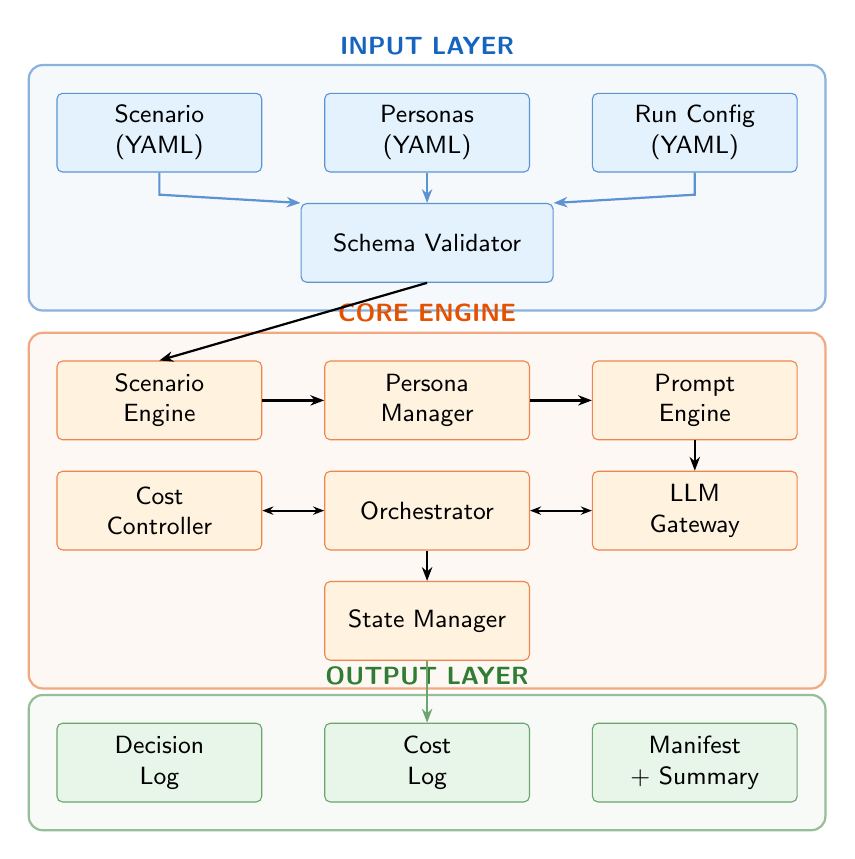
\begin{tikzpicture}[
    node distance=0.6cm and 0.6cm,
    inputbox/.style={rectangle, draw=accentblue!70, fill=inputcolor, rounded corners=2pt,
                     minimum height=1cm, minimum width=2.6cm, align=center, font=\small\sffamily},
    corebox/.style={rectangle, draw=accentorange!70, fill=corecolor, rounded corners=2pt,
                    minimum height=1cm, minimum width=2.6cm, align=center, font=\small\sffamily},
    outbox/.style={rectangle, draw=accentgreen!70, fill=outputcolor, rounded corners=2pt,
                   minimum height=1cm, minimum width=2.6cm, align=center, font=\small\sffamily},
    layerframe/.style={rectangle, draw=#1!50, fill=#1!4, rounded corners=5pt, inner sep=10pt, line width=0.8pt},
    arr/.style={-{Stealth[length=5pt]}, thick},
    dualarr/.style={{Stealth[length=4pt]}-{Stealth[length=4pt]}, thick},
]
    % ── Coordinates: 3-column grid ──
    \def\colA{0}
    \def\colB{3.4}
    \def\colC{6.8}

    % ── INPUT LAYER ──
    \node[inputbox] (sc)  at (\colA, 0)     {Scenario\\(YAML)};
    \node[inputbox] (pe)  at (\colB, 0)     {Personas\\(YAML)};
    \node[inputbox] (rc)  at (\colC, 0)     {Run Config\\(YAML)};
    \node[inputbox, minimum width=3.2cm] (val) at (\colB, -1.4) {Schema Validator};

    \begin{scope}[on background layer]
        \node[layerframe=accentblue, fit=(sc)(pe)(rc)(val),
              label={[font=\small\sffamily\bfseries, text=accentblue]above:INPUT LAYER}] {};
    \end{scope}

    % Arrows: converge to validator
    \draw[arr, accentblue!70] (sc.south) -- ([yshift=3pt]val.north-|sc) -- (val.north-|val.west);
    \draw[arr, accentblue!70] (pe.south) -- (val.north);
    \draw[arr, accentblue!70] (rc.south) -- ([yshift=3pt]val.north-|rc) -- (val.north-|val.east);

    % ── CORE ENGINE ──
    \node[corebox] (se)   at (\colA, -3.4)  {Scenario\\Engine};
    \node[corebox] (pm)   at (\colB, -3.4)  {Persona\\Manager};
    \node[corebox] (pr)   at (\colC, -3.4)  {Prompt\\Engine};

    \node[corebox] (cc)   at (\colA, -4.8)  {Cost\\Controller};
    \node[corebox] (orch) at (\colB, -4.8)  {Orchestrator};
    \node[corebox] (gw)   at (\colC, -4.8)  {LLM\\Gateway};

    \node[corebox, minimum width=2.6cm] (st) at (\colB, -6.2) {State Manager};

    \begin{scope}[on background layer]
        \node[layerframe=accentorange, fit=(se)(pm)(pr)(cc)(orch)(gw)(st),
              label={[font=\small\sffamily\bfseries, text=accentorange]above:CORE ENGINE}] {};
    \end{scope}

    % Core arrows: top row
    \draw[arr] (se) -- (pm);
    \draw[arr] (pm) -- (pr);

    % Core arrows: vertical connections
    \draw[arr] (pr) -- (gw);

    % Core arrows: middle row
    \draw[dualarr] (cc) -- (orch);
    \draw[dualarr] (orch) -- (gw);

    % Core arrows: to state
    \draw[arr] (orch) -- (st);

    % Validator to Scenario Engine
    \draw[arr] (val.south) -- (se.north);

    % ── OUTPUT LAYER ──
    \node[outbox] (dl) at (\colA, -8.0) {Decision\\Log};
    \node[outbox] (cl) at (\colB, -8.0) {Cost\\Log};
    \node[outbox] (mn) at (\colC, -8.0) {Manifest\\+ Summary};

    \begin{scope}[on background layer]
        \node[layerframe=accentgreen, fit=(dl)(cl)(mn),
              label={[font=\small\sffamily\bfseries, text=accentgreen]above:OUTPUT LAYER}] {};
    \end{scope}

    % State to output
    \draw[arr, accentgreen!70] (st) -- (cl);

\end{tikzpicture}
\caption{Three-layer framework architecture.}
\label{fig:arch}
\end{figure}

\subsection*{Input Layer}

Three YAML configuration files define a simulation, each validated against a JSON Schema:
\begin{itemize}
    \item \textbf{Scenario definition}: stakeholder roles, interaction rules (topology, round logic, visibility), incentive mechanisms, target metrics, and global constraints.
    \item \textbf{Persona definitions}: per-agent background, goals, risk profile, weighted decision factors, and personality traits. Separated from the scenario to enable reuse and combinatorial studies.
    \item \textbf{Run configuration}: LLM provider selection, model routing rules, retry logic, cost budgets, caching strategy, parallelism, and seed.
\end{itemize}

\subsection*{Core Engine}

The core engine consists of six components:
\begin{enumerate}
    \item \textbf{Scenario Engine}: parses and validates the input files, resolves persona-to-role assignments (seeded for reproducibility).
    \item \textbf{Persona Manager}: instantiates agents by rendering system prompts from persona definitions and scenario context using Jinja2 templates.
    \item \textbf{Interaction Orchestrator}: executes the simulation loop for each round: build per-agent context, render prompts, issue LLM calls (parallel or sequential), parse and validate responses, update immutable state, log results, and check termination conditions. Supports configurable topologies (\texttt{all\_to\_all}, \texttt{pairwise}, \texttt{hub\_spoke}, \texttt{custom}).
    \item \textbf{LLM Gateway}: unified provider interface built on \texttt{litellm}, providing transparent access to OpenAI, Anthropic, Mistral, and local models (Ollama). Includes cache lookup, model routing, and budget enforcement before each call.
    \item \textbf{Cost Controller}: tracks token usage and cost per API call, enforces hard budget limits, and triggers warnings or aborts at configurable thresholds.
    \item \textbf{State Manager}: maintains immutable per-round state snapshots, enabling full traceability and safe parallelization.
\end{enumerate}

\subsection*{Output Layer}

Structured outputs include:
\begin{itemize}
    \item \textbf{Decision logs} (JSONL): one entry per agent per round, including the decision, reasoning, token usage, cost, latency, and model used.
    \item \textbf{Cost logs} (JSONL): granular per-call cost tracking with cache hit status.
    \item \textbf{Reproducibility manifest} (JSON): config hash (SHA-256 over canonical inputs), seed, framework version, Git commit, dependency lock hash, and exact LLM model versions used.
    \item \textbf{Run summary} (JSON): aggregated results across repetitions (e.g., acceptance rates per persona, cost per simulation).
    \item \textbf{Config snapshot}: exact copy of all input files for full reproducibility.
\end{itemize}

\subsection*{Key Cost Optimization Strategies}

\begin{table}[H]
    \centering
    \small
    \begin{tabularx}{\textwidth}{lXr}
        \toprule
        \textbf{Strategy} & \textbf{Mechanism} & \textbf{Est.\ Impact} \\
        \midrule
        Structured output    & JSON mode / tool-use to eliminate parse retries              & $-$5--15\% calls \\
        Prompt compression   & Summarize history in late rounds                             & $-$30--60\% tokens \\
        Model routing        & Strong model for decisions, cheap for summaries               & $-$40--70\% sub-tasks \\
        Response caching     & SHA-256 hash over prompt $\to$ cache lookup                   & effective at $n{>}1$ reps \\
        Batch API            & OpenAI Batch API (50\% discount, 24h SLA)                    & $-$50\% if async OK \\
        Local models         & Ollama for development and testing                            & \$0 during dev \\
        \bottomrule
    \end{tabularx}
    \caption{Cost optimization strategies (exact measurements are part of the evaluation).}
    \label{tab:cost}
\end{table}

A detailed technical specification with full schema examples, data flow diagrams, and pseudocode is provided in a separate architecture document.

% ══════════════════════════════════════════════════════════
\section{Primary Use Case: Peatland Rewetting}
\label{sec:usecase}
% ══════════════════════════════════════════════════════════

The framework is demonstrated and evaluated using a concrete use case from climate policy and land use:

\textbf{Context.} In Germany and across Europe, large peatland areas have been drained for agricultural use. Drained peatlands emit substantial amounts of CO\textsubscript{2}, making them significant greenhouse gas sources. Rewetting these areas is an effective climate protection measure but requires landowners to abandon or adapt their current farming practices.

\textbf{Stakeholders.} The scenario comprises multiple actor groups with heterogeneous interests:
\begin{itemize}
    \item \textbf{Farmers} (diverse personas): conventional large-scale farms heavily dependent on arable farming, smaller diversified farms, ecologically oriented farmers, risk-averse vs.\ risk-seeking operators.
    \item \textbf{Public authorities}: municipalities, state agencies, or federal ministries offering compensation payments, subsidies, or regulatory requirements.
    \item \textbf{Environmental organizations}: NGOs exerting moral and public pressure but also offering cooperation.
\end{itemize}

\textbf{Research question.} Which combination of incentive mechanisms (compensation level, contract duration, transition support, paludiculture consultation, regulatory pressure) leads to acceptance of rewetting among which farmer personas? How do results change under variation of incentive parameters?

\textbf{Scope.} This scenario serves primarily as a \textit{technical demonstration} of the framework. The substantive validity of results (i.e., whether LLM agents accurately represent real farmers) is \textit{not} the core of this computer science thesis, but will be discussed as a plausibility check and identified as a starting point for domain-specific follow-up research.

% ══════════════════════════════════════════════════════════
\section{Related Work and Differentiation}
% ══════════════════════════════════════════════════════════

\begin{table}[h!]
    \centering
    \small
    \begin{tabularx}{\textwidth}{lp{3.5cm}X}
        \toprule
        \textbf{Framework / Work} & \textbf{Focus} & \textbf{Differentiation of This Thesis} \\
        \midrule
        AutoGen~\cite{wu2023}
            & Multi-agent conversations for software tasks
            & No focus on scientific simulation, no cost optimization \\
        CrewAI
            & Task-oriented agent teams
            & Workflow orchestration, not scientific reproducibility \\
        CAMEL~\cite{li2023}
            & Communicative agents
            & Role-playing focused, no economic evaluation \\
        Horton~\cite{horton2023}
            & LLMs as economic agents
            & Individual experiments, no framework \\
        ABM prototype (advisor)
            & Gift-exchange simulation
            & Domain-specific, single provider, no cost optimization \\
        \midrule
        \textbf{This thesis}
            & \textbf{Generic, cost-optimized simulation framework}
            & \textbf{Declarative, multi-provider, cost-optimized, reproducible} \\
        \bottomrule
    \end{tabularx}
    \caption{Differentiation from related work.}
    \label{tab:related}
\end{table}

% ══════════════════════════════════════════════════════════
\section{Preliminary Thesis Outline}
% ══════════════════════════════════════════════════════════

\begin{enumerate}
    \item \textbf{Introduction}
    \begin{enumerate}[label=\arabic{enumi}.\arabic*]
        \item Motivation and problem statement
        \item Objectives and research questions
        \item Structure of the thesis
    \end{enumerate}

    \item \textbf{Foundations}
    \begin{enumerate}[label=\arabic{enumi}.\arabic*]
        \item Large Language Models: architecture, APIs, cost models
        \item Agent-based modeling (ABM)
        \item Game theory and stakeholder negotiations
        \item Evaluation of LLM agents: validity, reproducibility
        \item Domain context: peatland drainage, climate policy, and incentive mechanisms
    \end{enumerate}

    \item \textbf{Related Work}
    \begin{enumerate}[label=\arabic{enumi}.\arabic*]
        \item LLMs as simulated economic actors
        \item Multi-agent frameworks (AutoGen, CrewAI, LangGraph, CAMEL)
        \item Cost optimization for LLM applications
        \item Research gap and contribution of this thesis
    \end{enumerate}

    \item \textbf{Requirements Analysis}
    \begin{enumerate}[label=\arabic{enumi}.\arabic*]
        \item Functional requirements
        \item Non-functional requirements (cost, performance, reproducibility)
        \item Use case: peatland rewetting including stakeholders and incentives
        \item Benchmark scenarios from game theory
    \end{enumerate}

    \item \textbf{Framework Design}
    \begin{enumerate}[label=\arabic{enumi}.\arabic*]
        \item Architecture overview
        \item Scenario definition language (schema design)
        \item Agent lifecycle and persona modeling
        \item Interaction orchestration and topologies
        \item LLM abstraction layer and multi-provider integration
        \item Cost optimization strategies
        \item Analysis and reporting pipeline
    \end{enumerate}

    \item \textbf{Implementation}
    \begin{enumerate}[label=\arabic{enumi}.\arabic*]
        \item Technology stack and project structure
        \item Core components and interfaces
        \item Prompt engineering strategies
        \item Caching, batching, and parallelization
        \item Test coverage and quality assurance
    \end{enumerate}

    \item \textbf{Evaluation}
    \begin{enumerate}[label=\arabic{enumi}.\arabic*]
        \item Experimental setup
        \item Use case: peatland rewetting simulation
        \item Benchmark results: validity in game-theoretic scenarios
        \item Cost analysis: optimized vs.\ baseline
        \item Performance benchmarks: latency and throughput
        \item Reproducibility analysis
        \item Discussion and limitations
    \end{enumerate}

    \item \textbf{Conclusion and Future Work}
    \begin{enumerate}[label=\arabic{enumi}.\arabic*]
        \item Summary of results
        \item Answers to research questions
        \item Limitations
        \item Outlook and future work
    \end{enumerate}
\end{enumerate}

% ══════════════════════════════════════════════════════════
\section{Preliminary Timeline}
% ══════════════════════════════════════════════════════════

\begin{table}[h!]
    \centering
    \begin{tabularx}{\textwidth}{llX}
        \toprule
        \textbf{Phase} & \textbf{Period} & \textbf{Tasks} \\
        \midrule
        1.\ Analysis
            & Month 1--2
            & Literature review, requirements analysis, domain analysis of peatland scenario, benchmark definition, analysis of prototype \\
        2.\ Design
            & Month 2--3
            & Architecture design, schema design, technology selection \\
        3.\ Implementation
            & Month 3--5
            & Core framework, persona modeling, LLM integration, cost optimizations, tests \\
        4.\ Evaluation
            & Month 4--5
            & Peatland scenario simulation, benchmark experiments, cost comparisons, sensitivity analyses \\
        5.\ Writing
            & Month 5--6
            & Writing, review, revision \\
        \bottomrule
    \end{tabularx}
    \caption{Preliminary timeline (assumption: 6-month thesis period).}
    \label{tab:timeline}
\end{table}

% ══════════════════════════════════════════════════════════
\section{Expected Contributions}
% ══════════════════════════════════════════════════════════

\begin{enumerate}
    \item \textbf{Practical contribution}: An open-source framework enabling researchers to run multi-stakeholder simulations via declarative configuration, demonstrated with the peatland rewetting use case.
    \item \textbf{Scientific contribution}: Systematic evaluation of cost optimization strategies for LLM agent systems with quantitative benchmarks.
    \item \textbf{Methodological contribution}: Design patterns and best practices for reproducible LLM-based experimental simulations, including a declarative persona schema.
    \item \textbf{Application contribution}: Exploratory results on which incentive mechanisms lead to acceptance of rewetting measures among different farmer types.
\end{enumerate}


% ══════════════════════════════════════════════════════════
% References
% ══════════════════════════════════════════════════════════

\begin{thebibliography}{99}

\bibitem{horton2023}
Horton, J.\,J. (2023).
\textit{Large Language Models as Simulated Economic Agents: What Can We Learn from Homo Silicus?}
NBER Working Paper No.\ 31122.

\bibitem{park2023}
Park, J.\,S., O'Brien, J.\,C., Cai, C.\,J., Morris, M.\,R., Liang, P. \& Bernstein, M.\,S. (2023).
Generative Agents: Interactive Simulacra of Human Behavior.
In: \textit{Proceedings of UIST~'23}.

\bibitem{aher2023}
Aher, G.\,V., Arriaga, R.\,I. \& Kalai, A.\,T. (2023).
Using Large Language Models to Simulate Multiple Humans and Replicate Human Subject Studies.
In: \textit{Proceedings of ICML~'23}.

\bibitem{li2023}
Li, G., Hammoud, H.\,A.\,A.\,K., Itani, H., Khizbullin, D. \& Ghanem, B. (2023).
CAMEL: Communicative Agents for ``Mind'' Exploration of Large Language Model Society.
In: \textit{Proceedings of NeurIPS~'23}.

\bibitem{wu2023}
Wu, Q., Bansal, G., Zhang, J. et al. (2023).
AutoGen: Enabling Next-Gen LLM Applications via Multi-Agent Conversation.
\textit{arXiv preprint} arXiv:2308.08155.

\bibitem{hevner2004}
Hevner, A.\,R., March, S.\,T., Park, J. \& Ram, S. (2004).
Design Science in Information Systems Research.
\textit{MIS Quarterly}, 28(1), 75--105.

\bibitem{teubner2025}
Teubner, T. \& Camacho, S. (2025).
[Reference for gift-exchange studies with LLMs].

\bibitem{chen2023}
Chen, L., Zaharia, M. \& Zou, J. (2023).
FrugalGPT: How to Use Large Language Models While Reducing Cost and Improving Performance.
\textit{arXiv preprint} arXiv:2305.05176.

\end{thebibliography}

\end{document}
